\documentclass[a4paper, 12pt, titlepage]{article}

% Including needed packages
\usepackage[margin=2cm]{geometry}
\usepackage{amsmath}
\usepackage{graphicx}
\usepackage{subfig}
\usepackage{float}

\title
{{\em Machine learning lab course}\\
Problem set 1: PCA, LLE, outlier detection}
\author{ROHRMANN Till, Matrnr: 343756}
\date{\today}

\begin{document}

\maketitle

\setcounter{section}{1}
\section{Application}

\subsection*{Assignment 4}

\subsubsection*{Original data}

\begin{figure}[H]
	\centering
	\subfloat[\label{l0}]{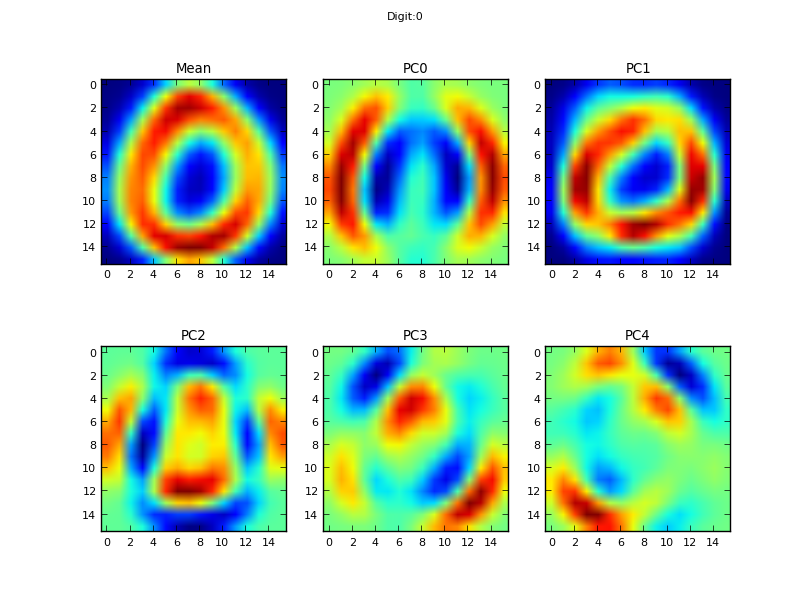
\includegraphics[width=12cm]{images/0.png}}\\
	\subfloat[\label{l0pvs}]{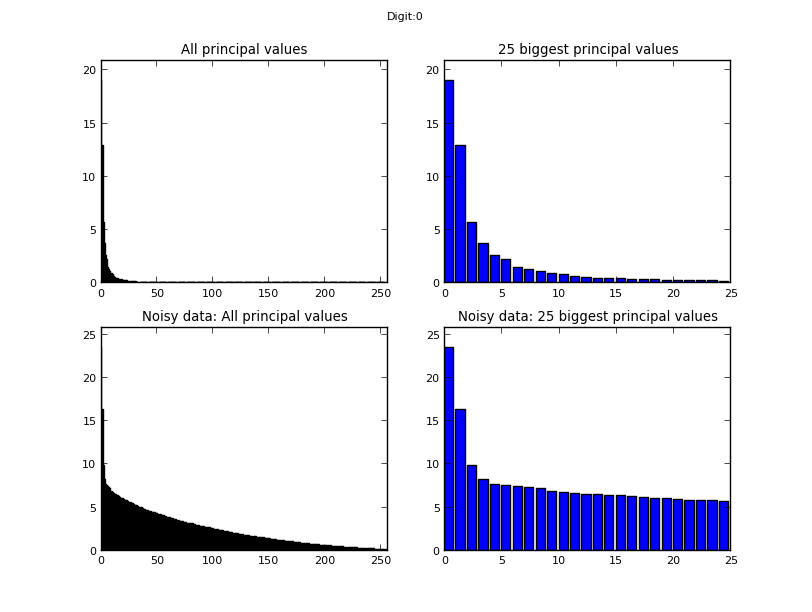
\includegraphics[width=12cm]{images/0pvs.png}}
	\caption{\protect\subref{l0} Mean and the first 5 principal components of the digit 0. \protect\subref{l0pvs} Top row: All principal values and the 25 biggest principal values of the digit 0. Bottom row: All principal values and the 25 biggest principal values of the noisy data of digit 0.}
\end{figure}

\begin{figure}[H]
	\centering
	\subfloat[\label{l1}]{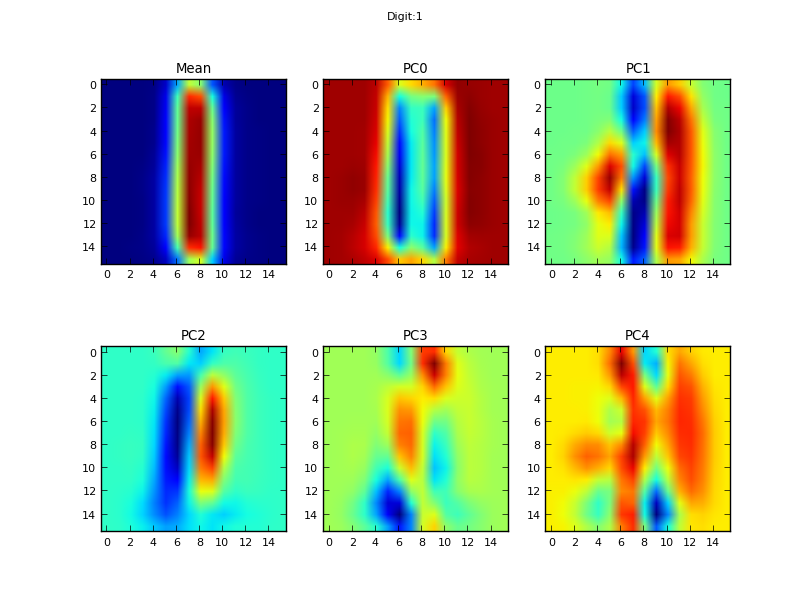
\includegraphics[width=12cm]{images/1.png}}\\
	\subfloat[\label{l1pvs}]{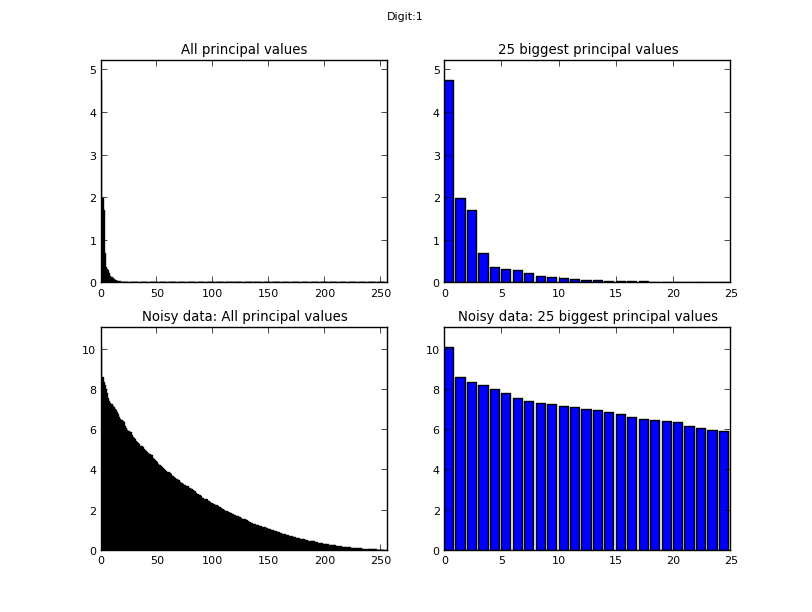
\includegraphics[width=12cm]{images/1pvs.png}}
	\caption{\protect\subref{l1} Mean and the first 5 principal components of the digit 1. \protect\subref{l1pvs} Top row: All principal values and the 25 biggest principal values of the digit 1. Bottom row: All principal values and the 25 biggest principal values of the noisy data of digit 1.}
\end{figure}

\begin{figure}[H]
	\centering
	\subfloat[\label{l2}]{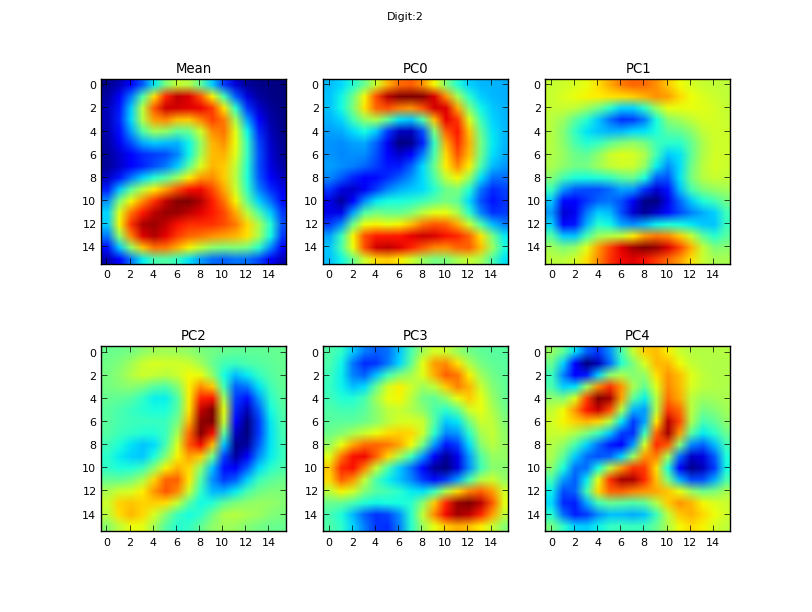
\includegraphics[width=12cm]{images/2.png}}\\
	\subfloat[\label{l2pvs}]{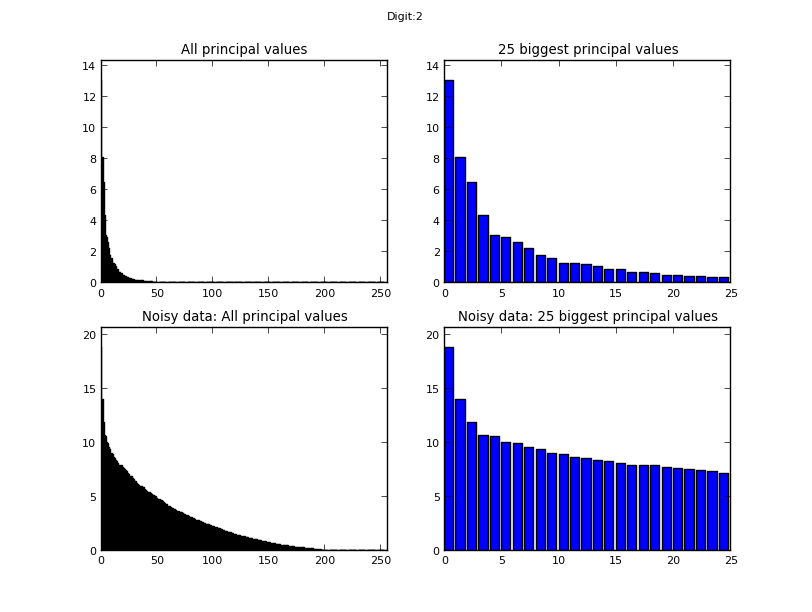
\includegraphics[width=12cm]{images/2pvs.png}}
	\caption{\protect\subref{l2} Mean and the first 5 principal components of the digit 2. \protect\subref{l2pvs} Top row: All principal values and the 25 biggest principal values of the digit 2. Bottom row: All principal values and the 25 biggest principal values of the noisy data of digit 2.}
\end{figure}

\begin{figure}[H]
	\centering
	\subfloat[\label{l3}]{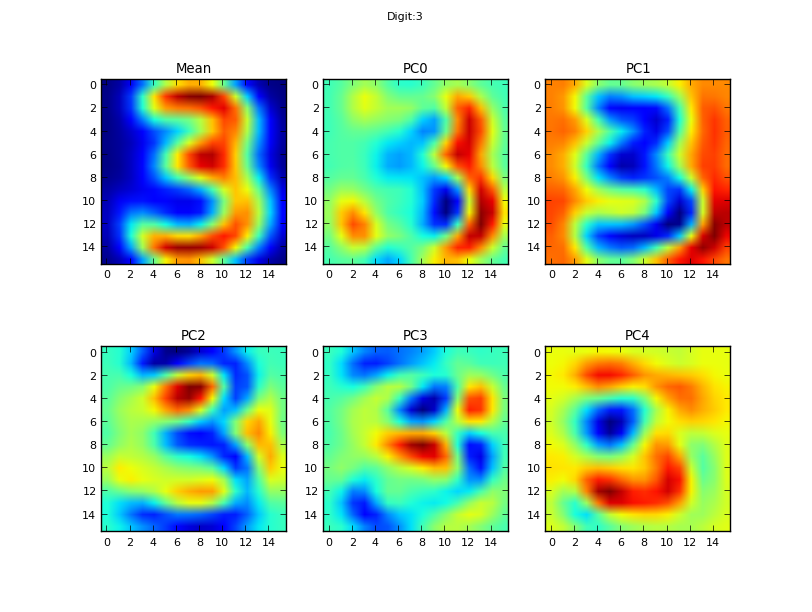
\includegraphics[width=12cm]{images/3.png}}\\
	\subfloat[\label{l3pvs}]{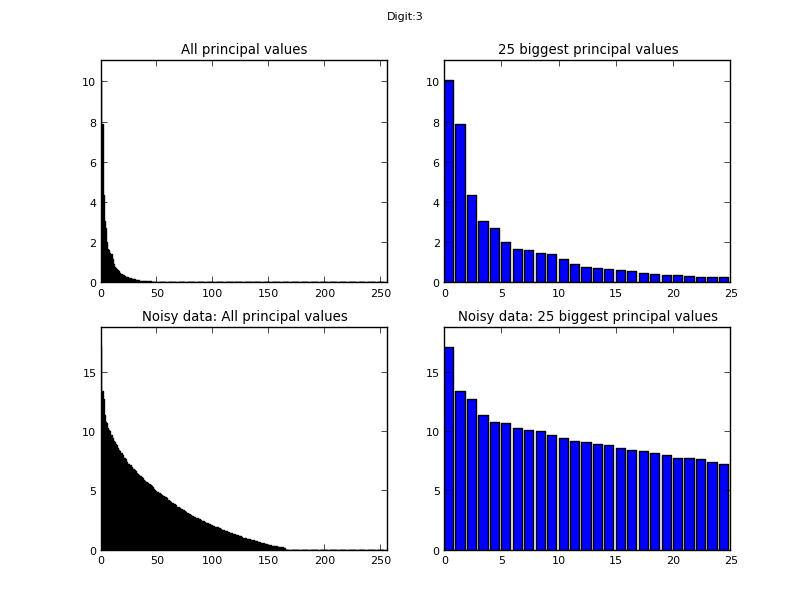
\includegraphics[width=12cm]{images/3pvs.png}}
	\caption{\protect\subref{l3} Mean and the first 5 principal components of the digit 3. \protect\subref{l3pvs} Top row: All principal values and the 25 biggest principal values of the digit 3. Bottom row: All principal values and the 25 biggest principal values of the noisy data of digit 3.}
\end{figure}

\begin{figure}[H]
	\centering
	\subfloat[\label{l4}]{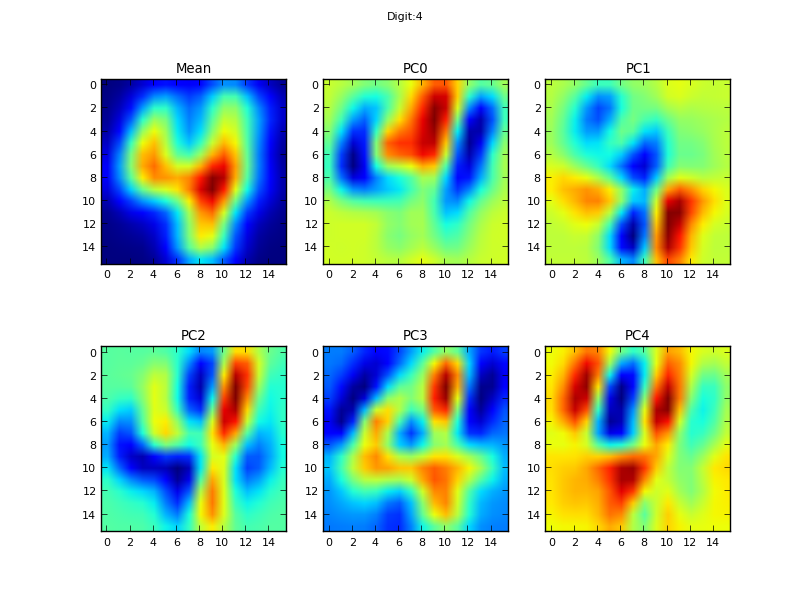
\includegraphics[width=12cm]{images/4.png}}\\
	\subfloat[\label{l4pvs}]{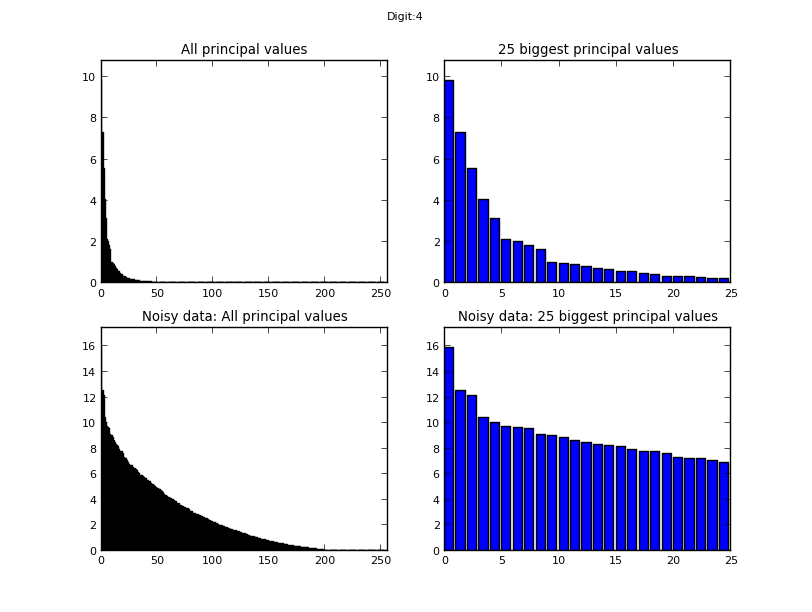
\includegraphics[width=12cm]{images/4pvs.png}}
	\caption{\protect\subref{l4} Mean and the first 5 principal components of the digit 4. \protect\subref{l4pvs} Top row: All principal values and the 25 biggest principal values of the digit 4. Bottom row: All principal values and the 25 biggest principal values of the noisy data of digit 4.}
\end{figure}

\begin{figure}[H]
	\centering
	\subfloat[\label{l5}]{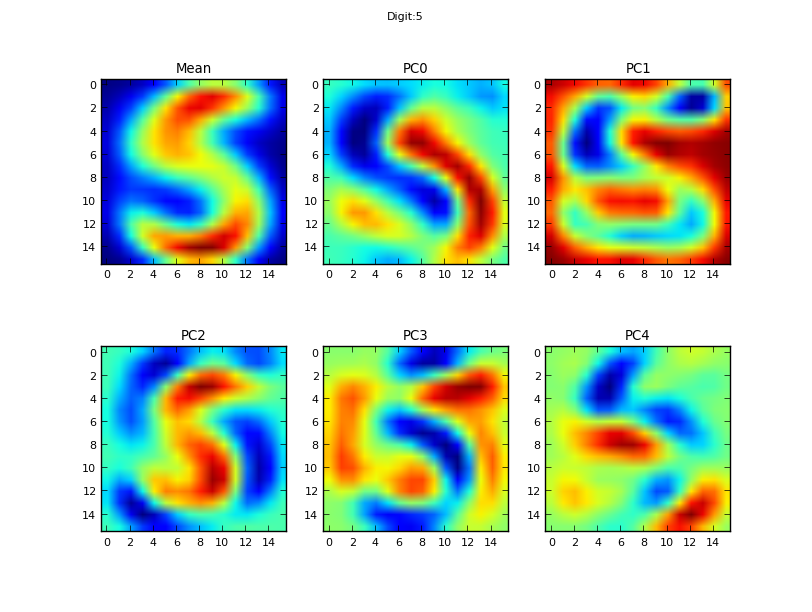
\includegraphics[width=12cm]{images/5.png}}\\
	\subfloat[\label{l5pvs}]{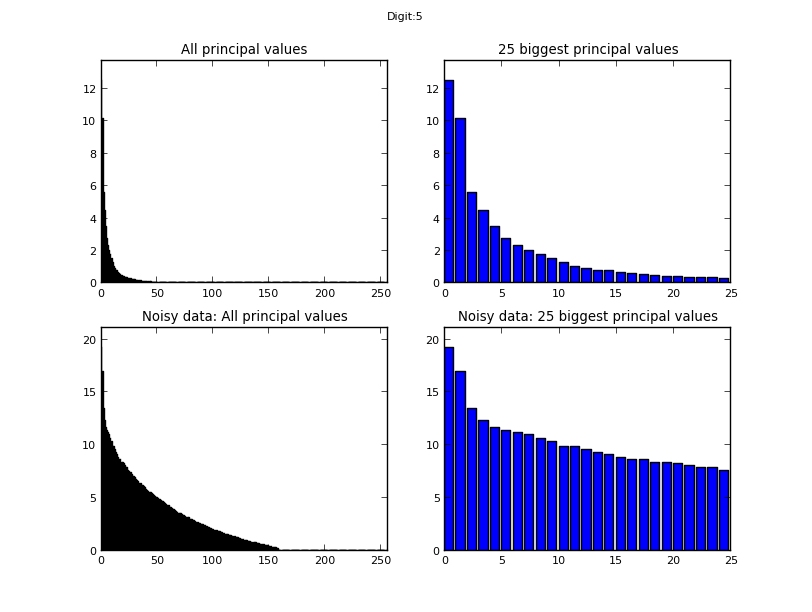
\includegraphics[width=12cm]{images/5pvs.png}}
	\caption{\protect\subref{l5} Mean and the first 5 principal components of the digit 5. \protect\subref{l5pvs} Top row: All principal values and the 25 biggest principal values of the digit 5. Bottom row: All principal values and the 25 biggest principal values of the noisy data of digit 5.}
\end{figure}

\begin{figure}[H]
	\centering
	\subfloat[\label{l6}]{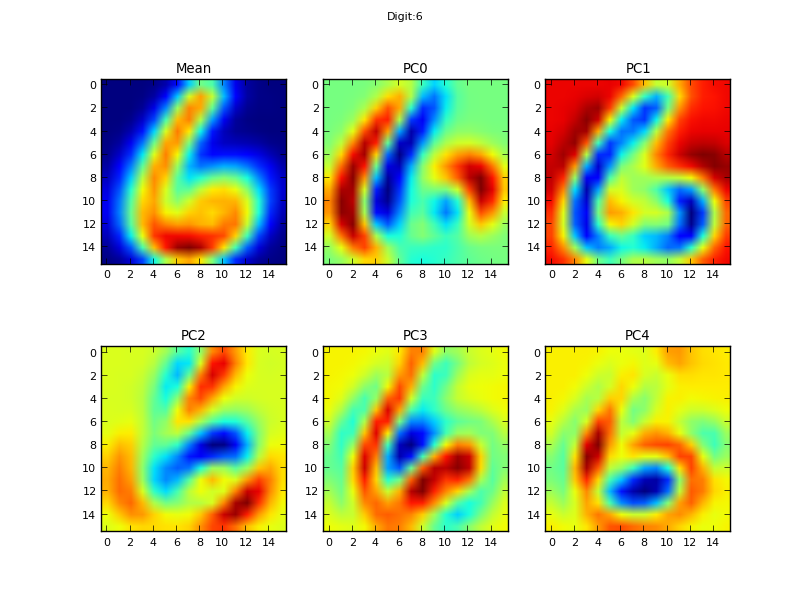
\includegraphics[width=12cm]{images/6.png}}\\
	\subfloat[\label{l6pvs}]{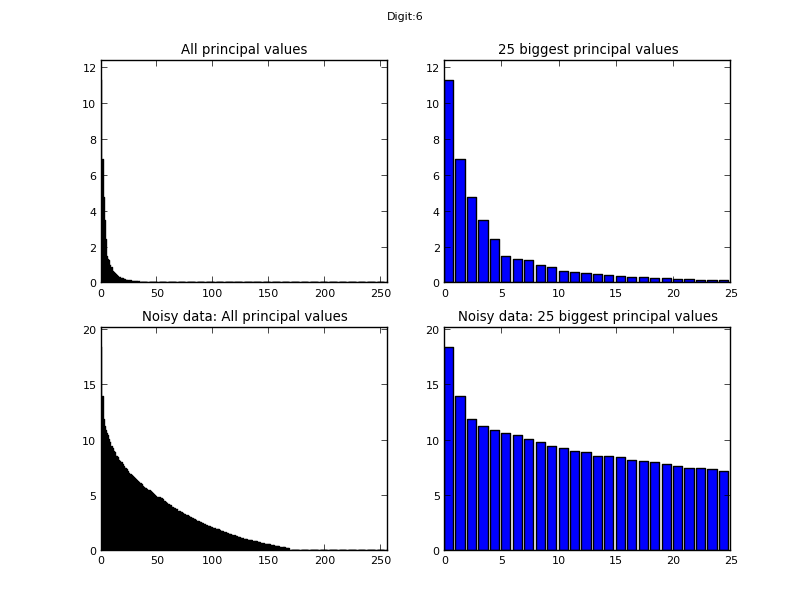
\includegraphics[width=12cm]{images/6pvs.png}}
	\caption{\protect\subref{l6} Mean and the first 5 principal components of the digit 6. \protect\subref{l6pvs} Top row: All principal values and the 25 biggest principal values of the digit 6. Bottom row: All principal values and the 25 biggest principal values of the noisy data of digit 6.}
\end{figure}

\begin{figure}[H]
	\centering
	\subfloat[\label{l7}]{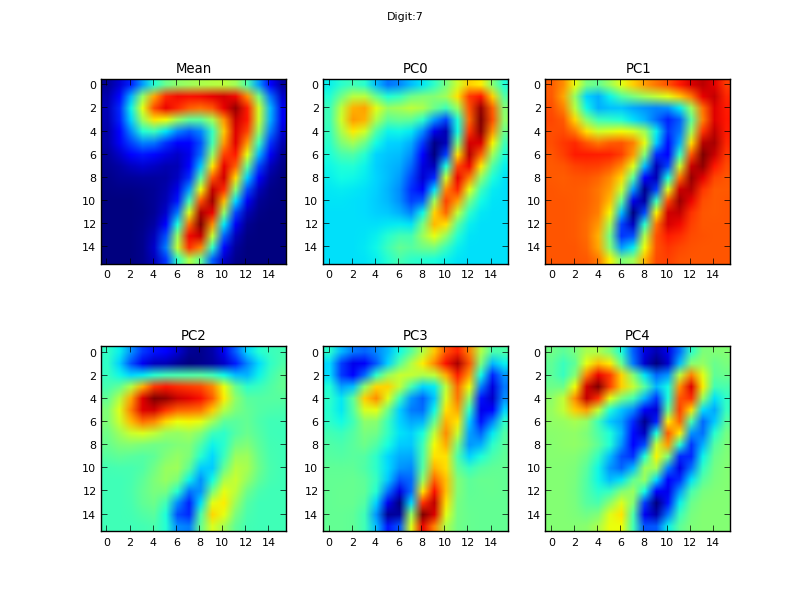
\includegraphics[width=12cm]{images/7.png}}\\
	\subfloat[\label{l7pvs}]{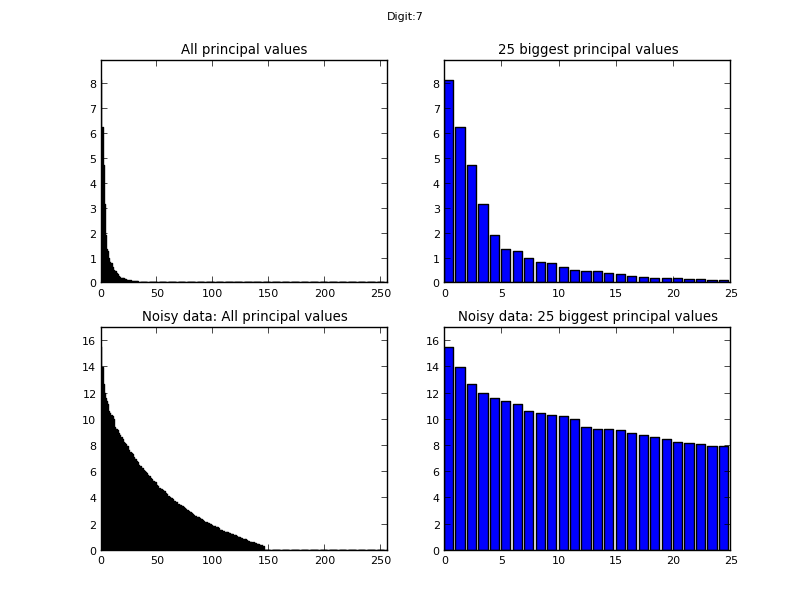
\includegraphics[width=12cm]{images/7pvs.png}}
	\caption{\protect\subref{l7} Mean and the first 5 principal components of the digit 7. \protect\subref{l7pvs} Top row: All principal values and the 25 biggest principal values of the digit 7. Bottom row: All principal values and the 25 biggest principal values of the noisy data of digit 7.}
\end{figure}

\begin{figure}[H]
	\centering
	\subfloat[\label{l8}]{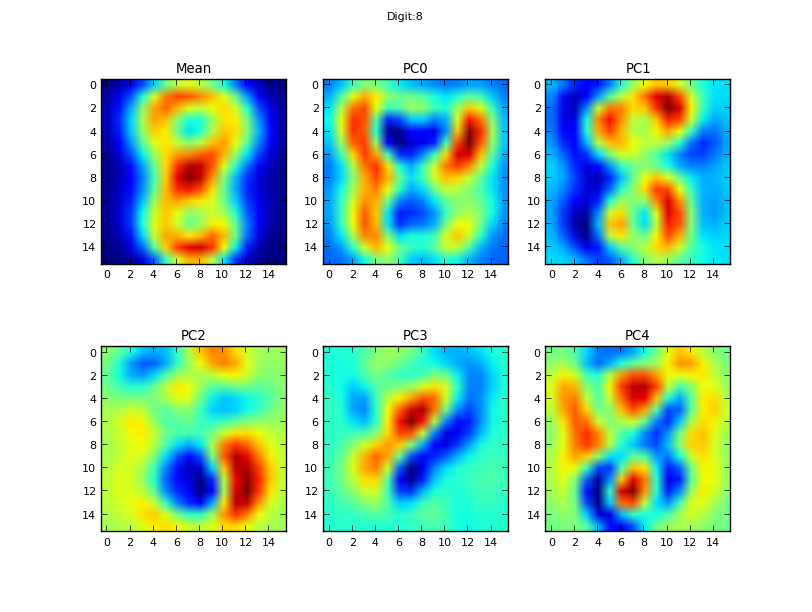
\includegraphics[width=12cm]{images/8.png}}\\
	\subfloat[\label{l8pvs}]{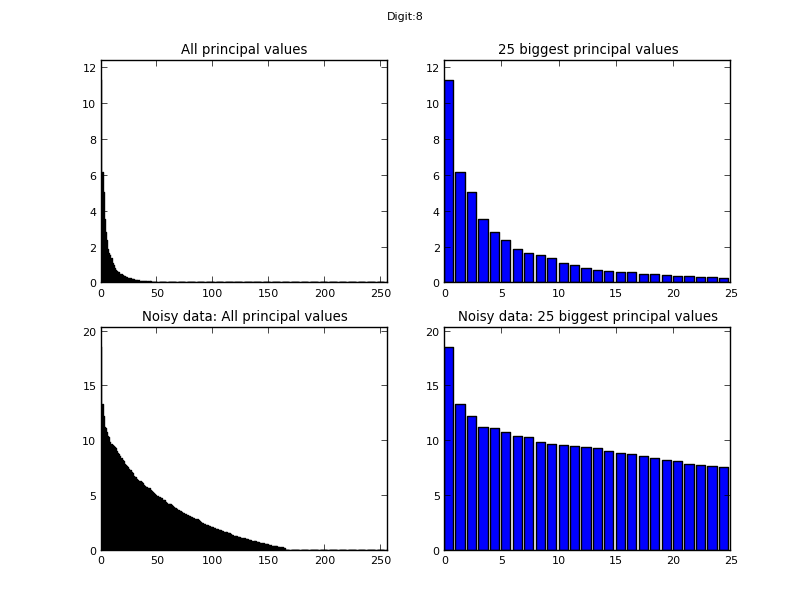
\includegraphics[width=12cm]{images/8pvs.png}}
	\caption{\protect\subref{l8} Mean and the first 5 principal components of the digit 8. \protect\subref{l8pvs} Top row: All principal values and the 25 biggest principal values of the digit 8. Bottom row: All principal values and the 25 biggest principal values of the noisy data of digit 8.}
\end{figure}

	
\begin{figure}[H]
	\centering
	\subfloat[\label{l9}]{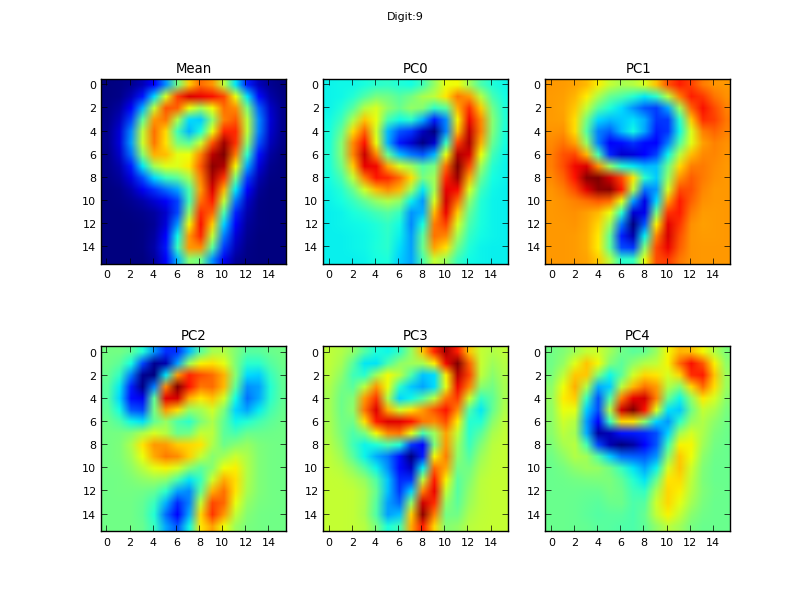
\includegraphics[width=12cm]{images/9.png}}\\
	\subfloat[\label{l9pvs}]{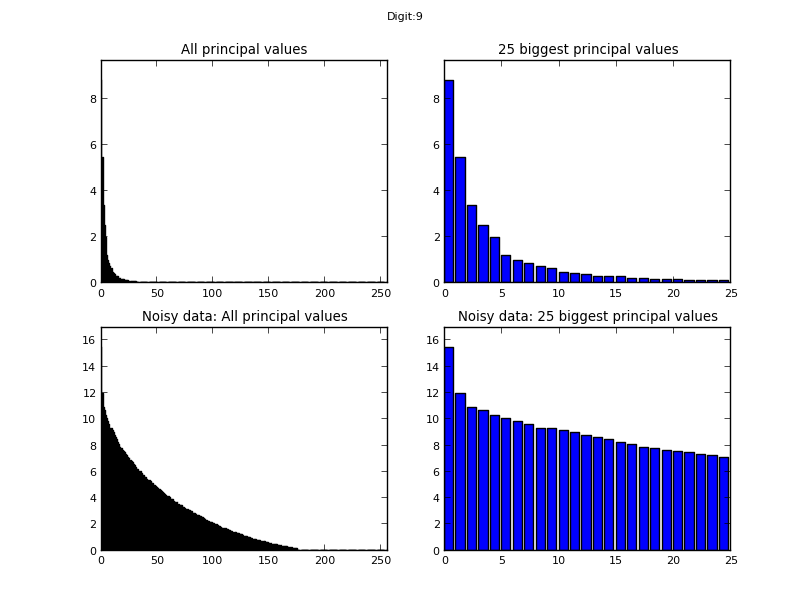
\includegraphics[width=12cm]{images/9pvs.png}}
	\caption{\protect\subref{l9} Mean and the first 5 principal components of the digit 9. \protect\subref{l9pvs} Top row: All principal values and the 25 biggest principal values of the digit 9. Bottom row: All principal values and the 25 biggest principal values of the noisy data of digit 9.}
\end{figure}

\subsubsection*{Noisy data}

In the following a Gaussian noise with a variance $\sigma^2=2.25$ has been added to the original data.
For the noisy data we observe that the principle values increase.
This is not surprising because what we have done is the following:
We added to each dimension $X_d$ a Gaussian white noise $W_d$ with $0\le d < 256$ denoting the dimension.
All $W_d$ are independent random variables and Gaussian.
Thus they maintain this property under rotations as well.
Therefore adding independent white noise to the original data is the same as adding independent white noise to the projected data in the coordinate system spanned by the principle components.
Let $\tilde{X}_d$ denote the coordinates in the new coordinate system.
Then is the perturbed value $\hat{X}_d = \tilde{X}_d + W_d$.
This means for the variance $Var(\hat{X}_d) = Var(\tilde{X}_d) + Var(W_d)$ where $Var(\tilde{X}_d)$ is the $d$th principal value and $Var(W_d)=\sigma^2$.
Adding white noise does not affect the covariance though: $Cov(\hat{X}_i,\hat{X}_j) = Cov(\tilde{X}_i,\tilde{X}_j) = 0$ with $i\not = j$.
To make a long story short: Adding Gaussian white noise which is independent, simply increases the principal values and thus the variances in the directions of the principal components by the variance of the white noise $\sigma^2$.
However, since we have only a comparatively small number of sampling points of our data in a highly dimensional space, the empirical covariance matrix of the white noise shows still some correlations between pairs of components and the variance of the individual components might differ as well.
That is the reason, why we still can observe that the principal values seem to converge against $0$ and not against variance of the white noise.
Furthermore this explains also why some of the components are influenced by a greater summand than others.

\subsubsection*{Denoising}

\begin{figure}[H]
	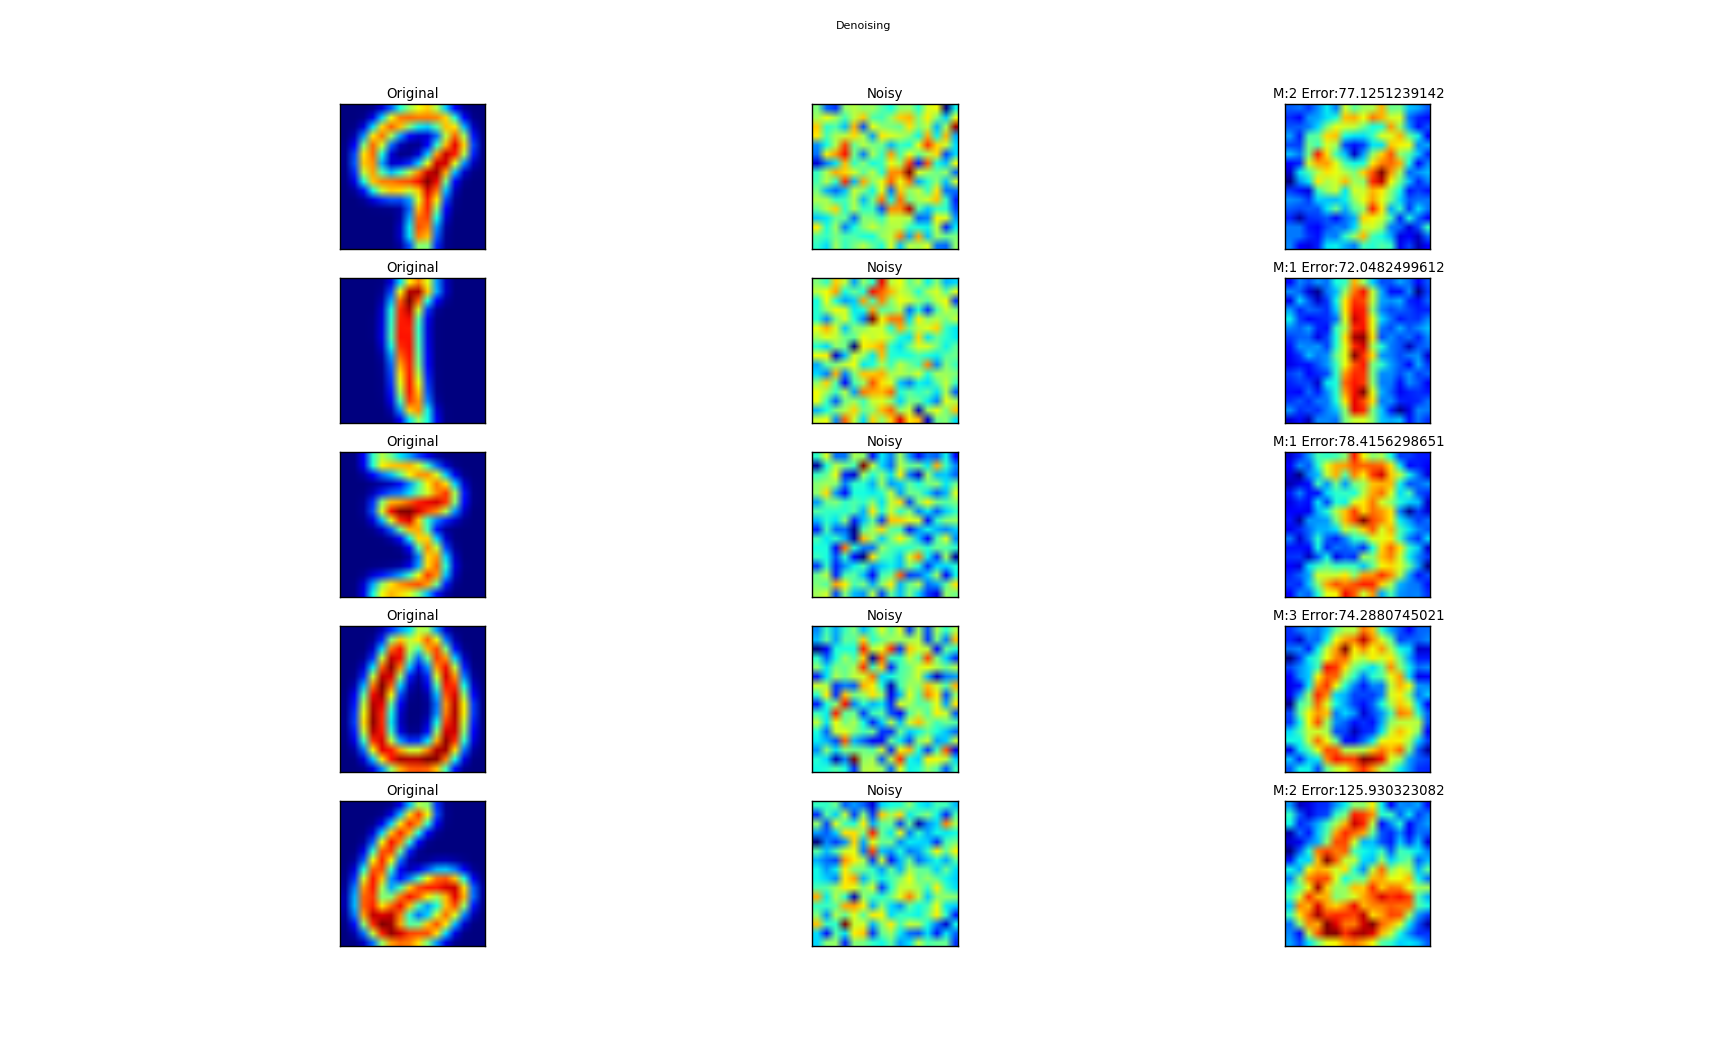
\includegraphics[width=20cm]{images/denoising.png}
	\caption{Left column shows the original images. Middle column shows the noisy images. Right column shows the denoised images with $M$ denoting the number of principle components used for the reconstruction.}
\end{figure}

\subsection*{Assignment 5}

\begin{figure}[H]
	\centering
	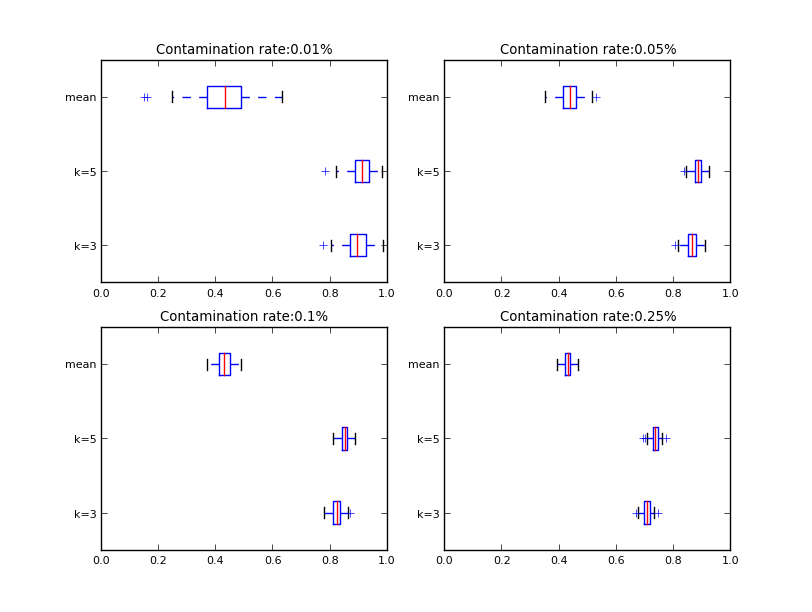
\includegraphics[width=17cm]{images/boxplot.png}
	\caption{Box plot showing the distribution of the AUCs values for different rates of contamination of the different outlier detection methods: Gamma index with $k=3$, Gamma index with $k=5$ and mean distance.}
\end{figure}

One clearly sees that the mean distance method has an AUC value whose mean is close to $0.5$ which means that this method is not well suited for the outlier detection in our case.
In contrast to that the gamma index methods perform far more better.
For moderate contamination rates, $0.01$ and $0.05$, they have an AUC value whose mean is close to $0.9$.
For higher contamination rates, their performance degrades slightly.
It is noteworthy that the gamme index method using $5$ neighbors performs marginally better than the same method using only $3$ neighbors.

\subsection*{Assignment 6}

\begin{figure}[H]
	\centering
	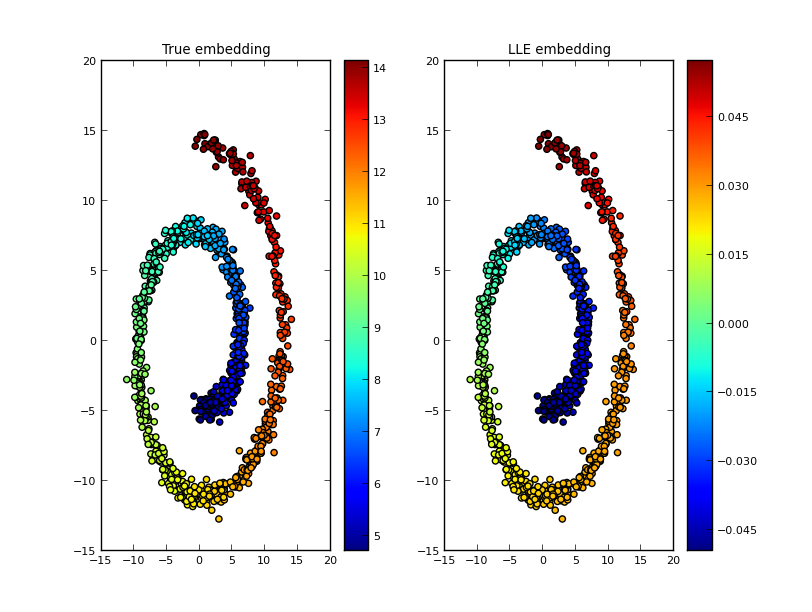
\includegraphics[width=17cm]{images/flatroll.png}
	\caption{Left: Original data with true embedding indicated by the coloring. 
	Right: Original data with the calculated LLE embedding indicated by the coloring.}
\end{figure}

\begin{figure}[H]
	\centering
	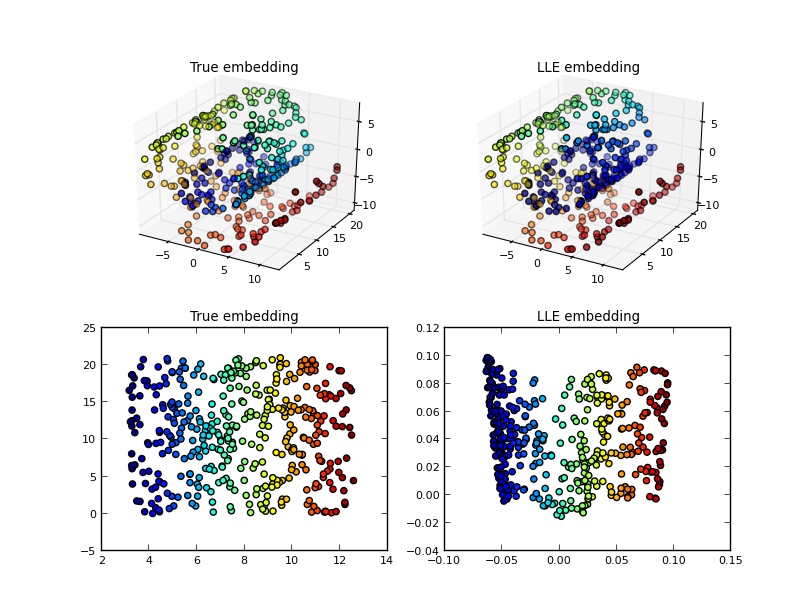
\includegraphics[width=17cm]{images/swissroll.png}
	\caption{Top left: Original data with true embedding.
	Bottom left: True 2D manifold with the same coloring as in the top left plot.
	Top right: Original data with calculated LLE embedding.
	Bottom right: Calculated 2D manifold with the same coloring as in the top right plot.}
\end{figure}

\begin{figure}[H]
	\centering
	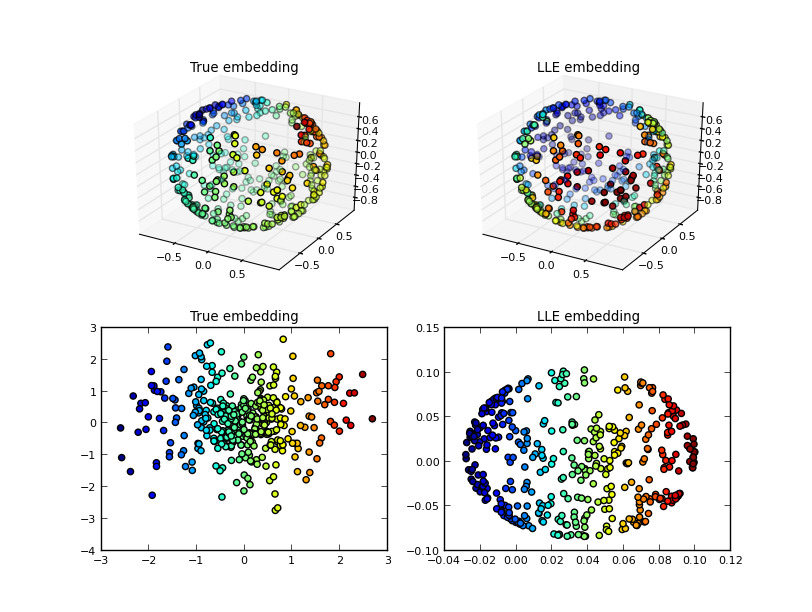
\includegraphics[width=17cm]{images/fishbowl.png}
	\caption{Top left: Original data with true embedding indicated by the coloring.
	Bottom left: True 2D manifold with the same coloring as in the top left plot.
	Top right: Original data with calculated LLE embedding.
	Bottom right: Calculated 2D manifold with the same coloring as in the top right plot.}
\end{figure}

\subsubsection*{Why is it diffcult to obtain an embedding in which the brink of the fishbowl is on the fringe of the embedding?}

In order to embed the fishbowl into a $2$-dimensional map, one has to widen the brink of the fishbowl, that is to say one has to stretch it to the outside. 
This causes inevitably a change in the neighborhood relations of those points (see the $2$-dimensional plot of the true embedding where the brink points are far less densely packed than in the LLE embedding).
Since LLE maintains the local neighborhood relations, this method has some problems finding a good embedding.

\subsubsection*{Why does the $eps-ball$ criterion appear to work better than the $knn$-criterion?}

With the $eps-ball$ criterion the brink points have fewer assigned neighbors than the points not lying close to the brink. Consequently, they also have fewer constraints to fulfill in the final $2$-dimensional embedding and thus they can be more easily placed on the fringe of the resulting embedding.

Nonetheless, I obtained the LLE-embedding with the $knn$ criterion and the result is also quite satisfying.
\subsection*{Assignment 6}

\begin{figure}[H]
	\centering
	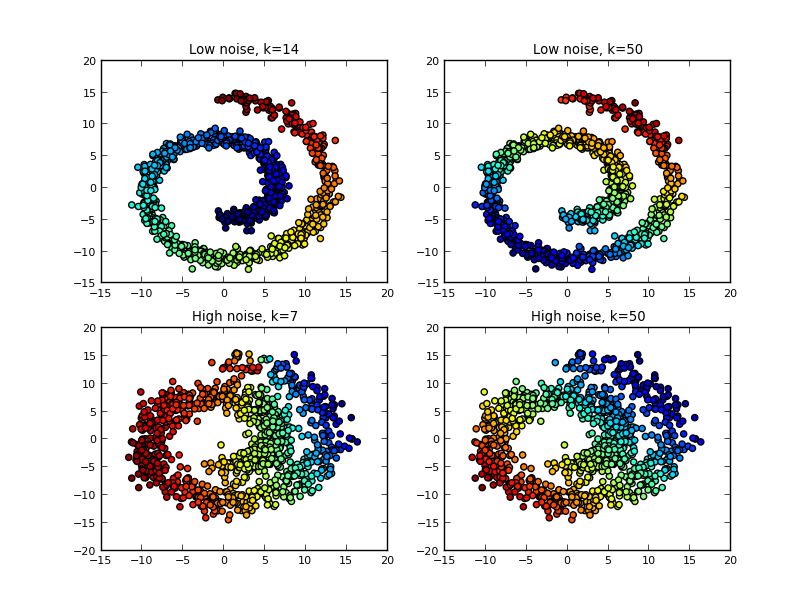
\includegraphics[width=17cm]{images/noisyFlatroll.png}
	\caption{Top left: LLE embedding with $k=14$ of flat roll with low noise.
	Top right: LLE embedding with $k=50$ of flat roll with low noise.
	Bottom left: LLE embedding with $k=7$ of flat roll with high noise.
	Bottom right: LLE embedding with $k=50$ of flat roll with high noise.}
\end{figure}

The figure shows that LLE can successfully retrieve the embedding of a flat roll which is affected by low noise.
However if one sets the number of neighbors too high, the embedding won't be found.
The same holds if the noise becomes too high.
In the bottom left image the chosen number of neighbors is the minimum such that the graph is still weakly connected.
But since the noise is so high that the roll starts to admix, the neighborhood structure cannot be retrieved correctly anymore.
Thus, rendering the lle method unusable in this case. 


\end{document}
